\chapter{How to use this template}
The goal of this template is to save you time (and effort) trying to put together your dissertation (hard enough as it is). This chapter covers many of the basics. 

\section{Overview}
This template uses multiple files to separate out chapters and major components as well as folders to neatly separate images. If this does not make your life easier, feel free to merge things later. All examples and instructions here assume the standard set up.

\begin{enumerate}
\item \texttt{titlepage.tex}. Fill this one out with all the relevant information for the title page. Make sure to comment out or delete anything you don't need. 
\item \texttt{preamble.tex}. You can load any additional packages you need here as well as create your own commands and macros. Some are already defined for you. Most things are handled by the .cls file, but you can change a few things here without breaking anything (hopefully). 
\begin{itemize}
\item A macro to add comments in color has been added for you. It can make revisions easier if you share your document with your advisor and you want the comments to show in the pdf. For example, here \PersonA{something should be changed in this section}. You can add as many as you like and modify the colors, names and commands.
\item You can format the bibliography. Initially it is set to sort numerically. If you'd like to change the name used for the bibliography (currently set to ``References'') adjust it in the options of \verb|\printbibliography| on \texttt{main.tex}.
\item The \LaTeX default is to indent almost every paragraph (all {\em except} for paragraphs immediatelly after a heading). If you would rather {\em not} indent {\em every} paragraph, add a \% symbol to comment out the \texttt{indentfirst} package (be warned ETD reviewers may not like it).
\item If you like to use hyperlinks, the \texttt{hyperref} package is loaded for you and initialized with {\color{pdflinkcolor}dark blue} for all links. As of Summer 2022, the ETD guidelines do not mention hyperlinks so there is no established standard for whether or not to use them or how to implement them. You may conceal links by setting all colors to black, or disable them altogether by just not loading the \texttt{hyperref} package.
\item The \texttt{cleveref} package is loaded to make references a bit easier (examples of how later on). As far as formatting goes, just know that if you create new environments they may not get referenced correctly until you feed \texttt{cleveref} the correct names.
\end{itemize}
\item \texttt{dedication.tex} You can (optionally) dedicate your dissertation to anyone and write acknowledgments here. 
\item \texttt{abstract.tex} Self-explanatory, for the abstract.
\item \texttt{chapter<n>.tex} Only two of these are included but add as many as you like. Just make sure to lead with \verb|\chapter{<title>}| on the first line of each file.
\item \texttt{appendix.tex} After the \verb|\appendix| command is called, any additional chpaters are treated as an appendix. You can choose to include them all in one file (if they are short) or as separate files (\texttt{appendix01.tex, appendix02.tex}, etc.)
\item \texttt{biblio.bib} Feel free to modify this if \texttt{biblatex} is not your thing, but the default is to load it in the .cls file (be aware in case you load something else) and refer to the \texttt{biblio.bib} file for information. You can usually download citations in .bib format and then modify the entries so they are easier to cite. 
\item \texttt{main.tex} Not a lot happens here. To keep things tidy, you can add new files with \verb|\input{<filename>}| commands.
\end{enumerate}

\section{Quick start}
Just a few things to keep in mind as you write things. 
\subsection{Chapter headings}
Chapter headings can be modified by loading different options for the document class in \texttt{main.tex}.

\lstinputlisting[firstline=1, lastline=1]{main.tex}

The option \texttt{boldcaps} most closely resembles the sample .pdf files posted on the ETD website (as of Summer 2022), though \texttt{boldheadings} should also be acceptable. For the boldface averse, there are also \texttt{allcaps} (which uses all caps headings for chapters) and \texttt{plainheadings} (\verb|\normalfont| throughout), though they may not match guidelines. You can also modify the font size here. 

\subsection{Title case and sentence case}
Chapter, section and subsection heading should use title case (Where Every Major Word is Capitalized), while everything else (subsubsection, paragraph, etc.) should use sentence case (Where only the first word and proper names are capitalized). Title case is implemented automatically. Note that while the title of this subsection is typed
\lstinputlisting[firstline=34, lastline=34]{chapter02.tex}
without any capital letters, it prints both in the heading and Table of Contents with correct capitalization. However, this setting does not affect subsubsections.

\subsubsection{Title case is not applied here}
\subsubsection{You should use sentence case when typing titles}

The suggested use is to type all sectioning titles in {\em sentence case}. If it needs to be adjusted to title case, it will be done automatically and it will otherwise be left as is. The settings can be adjusted from the preamble file. The current list is below.
\begin{lstlisting}
% List of words that will not be capitalized in Title Case
\Addlcwords{of, and, a, an, the, or, to, in, on, at}
\end{lstlisting}
If any words that should remain lower case are incorrectly capitalized, add them there.

\section{What if a section title is excessively long and does not fit into a single line no matter what you do?}
What \textit{should} happen is the section heading should run without hanging indents, so that even if it needs more than one line it's all flush left.
\subsection{How the table of contents handles these very long headings that do not fit in a single line}
The hanging indent is only in the main body. The table of contents should display the very long section/subsection title in separate lines, with the second one having a 0.25" indent. 
\subsubsection{Even very long titles should be moved to the next line down in the table of contents with an additional indent}
\subsection{Using math mode in headings, like  \texorpdfstring{$\mathbb{N}$}{N}}
Note that if you try to put math symbols in the title of a chapter, section, etc. you may get errors (or may run out of time waiting for the document to compile). Terms in math mode, like $(p,q)$ will automatically be capitalized unless you add them to the list of lowercase words in the preamble (look for \verb|\Addlcwords|). Otherwise, try what is written here:

\begin{lstlisting}
\texorpdfstring{<math symbol>}{<plain text alternative>}
\end{lstlisting}

\section{Floats}
There is a very good chance you will have to include figures in your dissertation. Note that you can add an optional position parameter when you include floating elements. If you don't include any, \LaTeX will decide the placement for you. You can always force an element to appear exactly where it is called with \texttt{[H]} or \texttt{[h!]}, but be aware that it prevents any empty spaces after the object from being filled with text that is typed after it. Just make sure that when you force empty space it doesn't take up more than half the page (5.5 inches) unless it's the end of a chapter. The options for positions are 
\begin{itemize}
\item \texttt{h} Here. A gentle suggestion.
\item \texttt{H} HERE. In shouty caps.
\item \texttt{t} Top, of the page.
\item \texttt{b} Bottom, self-explanatory.
\item \texttt{p} Page, meaning in a new page only for the float.
\item Adding an exclamation mark (\texttt{!}) to any of these overrides any choice \LaTeX would make on its own. Use sparingly.
\end{itemize}

The List of Tables and List of Figures entries should only contain the first sentence of the captions for each table/figure. To ensure this, make sure to use the following syntax when entering captions.
\begin{lstlisting}
\caption[<First sentence only.]{<Full caption.>}
\end{lstlisting}

\begin{sloppypar}
You will also have to be careful to use the \verb|\caption| and \verb|\label| commands in the right order. The \verb|\caption| command should be called \textit{after} figures (whether it is created with Tikz or inserted via \verb|\includegraphics| or similar) inside the \verb|\figure| environment and \textit{before} tables (before \verb|\tabular|, \verb|\tabu| or similar) inside the \verb|\table| environment.
\end{sloppypar}

\begin{figure}[h]
\begin{center}
\includegraphics[width=2in]{images/fig}
\end{center}
\caption[Write the first sentence in the caption here.]{Write the first sentence in the caption here. The rest of the caption can now follow. This is figure 1.}
\label{fig1}
\end{figure}

\begin{figure}[h]
\centering
\includegraphics[width=2in]{images/fig}
\caption[This is figure 2.]{This is figure 2. Also a fig.}
\label{fig2}
\end{figure}

To keep things tidy, all image files are kept in a folder. This means that the \verb|\includegraphics| command needs to have the parent directory (i.e. just typing \verb|\includegraphics{fig}| would not work). Just to show that it is an option, \Cref{fig3} was made with \texttt{PSTricks}. Bear in mind that projects with PSTricks should be compiled with XeLaTeX (pdfLaTeX will not recognize the commands) and that if opacity values are provided then TeX Live 2020 or 2022 should be used\footnote{A bug in the 2021 version ignores opacity. Should be fixed in the 2022 version whenever it comes out.}.

\begin{figure}[htpb]
\label{fig3}
\centering
\psscalebox{1.0 1.0} % Change this value to rescale the drawing.
{
\begin{pspicture}(0,-1.2888296)(9.298557,1.2888296)
\definecolor{colour1}{rgb}{0.2,0.2,1.0}
\psdots[linecolor=black, dotsize=0.2](0.4,-0.40972805)
\rput[bl](0.33,-0.2){$v_0$}
\psdots[linecolor=black, dotsize=0.2](2.8,-0.40972805)
\rput[bl](2.7,-0.2){$v_0$}
%\psdots[linecolor=black, dotsize=0.2](4.8,-0.40972805)
\rput[bl](4.75,-0.2){\textcolor{colour1}{$v_1$}}
\psdots[linecolor=colour1, dotsize=0.2](4.8,-0.40972805)
\psline[linecolor=colour1, linewidth=0.04, arrowsize=0.05291667cm 2.0,arrowlength=1.4,arrowinset=0.0]{->}(2.8,-0.40972805)(4.8,-0.40972805)
\psdots[linecolor=black, dotsize=0.2](7.2,-0.40972805)
\rput[bl](6.8,-0.2){$v_0$}
\psdots[linecolor=black, dotsize=0.2](9.2,-0.40972805)
\rput[bl](9.3,-0.2){$v_1$}
\psline[linecolor=black, linewidth=0.04, arrowsize=0.05291667cm 2.0,arrowlength=1.4,arrowinset=0.0]{->}(7.2,-0.40972805)(9.2,-0.40972805)
\psdots[linecolor=colour1, dotsize=0.2](8.2,1.190272)
\rput[bl](8.35,1.1){\textcolor{colour1}{$v_2$}}
\psline[linecolor=colour1, linewidth=0.04, arrowsize=0.05291667cm 2.0,arrowlength=1.4,arrowinset=0.0]{->}(7.2,-0.40972805)(8.2,1.190272)
\psline[linecolor=colour1, linewidth=0.04, arrowsize=0.05291667cm 2.0,arrowlength=1.4,arrowinset=0.0]{->}(9.2,-0.40972805)(8.2,1.190272)
\rput[bl](0.1,-1.209728){$\Delta^0$}
\rput[bl](3.55,-1.209728){$\Delta^1$}
\rput[bl](8,-1.209728){$\Delta^2$}
\end{pspicture}
}

\caption[This is figure 3.]{This is figure 3. Abstract figs created with \texttt{PSTricks}.}
\end{figure}

\begin{table}[h]
\caption[Here is a table.]{Here is a table. It is important for ETD that figure captions are \textbf{below} the table and table captions are \textbf{above}.}
\centering
\begin{tabular}{|l|l|}
\hline
a & table\\
\hline
goes& here\\
\hline
\end{tabular}
\end{table}
Here is some text to separate the tables and show the difference when you use \verb|\caption| before or after using the \verb|\tabular| environment.
\begin{table}[h]
\centering
\begin{tabular}{|l|l|}
\hline
a & table\\
\hline
goes& here\\
\hline
\end{tabular}
\caption[This caption is in the wrong position]{This caption is in the wrong position. Since vertical space has been reserved above the tables only, it will not look right.}
\end{table}

Figure \ref{fig1} is a fig. Compare the vertical spacing assigned to \cref{fig1} and \cref{fig2} before the caption. For figures and tables, \verb|\centering| adds less vertical padding. Use \verb|\begin{center}| and \verb|\end{center}| to enclose sections with more than one element that need to be centered. 

\section{Theorem environments}
Several theorem-like environments are pre-defined for you in \texttt{preamble.tex}. Here is one example of how to use them. Note that the optional argument \verb|<Theorem name>| appears in parentheses and can be used when using named theorems. 

\begin{Thm}[Theorem name]
\label{mythm}
This is a theorem.
\end{Thm}
\begin{proof}
This is the proof of the theorem above.
\end{proof}

\begin{Def}
This is a definition.
\end{Def}

\begin{Ex}
This is an example. 
\end{Ex}

When referring to environments, pay attention to where the label command is added, or else the references may not print correctly.

\section{Cross-references}
The \texttt{cleveref} package allows for easier references. Did you write a proposition that turned into a lemma? Instead of having to track down these changes and replacing ``proposition \verb|\ref{<label>}|'' with ``lemma \verb|\ref{<label>}|,'' use ``\verb|\cref{<label>}|. For example, this points to \cref{mythm}. The capitalized version exists too, \Cref{mythm}. Make sure the labels are inside the environments when you add them. In the case of figures, it's important that labels be added after captions. A reference to \Cref{fig3} fails here because the label is in the wrong place. 

All things you cite should be listed in \texttt{biblio.bib} and be given an easy-to-remember name. For example, we can cite a book here as \cite{sample}. 
